\documentclass[12pt,]{article}
\usepackage[utf8]{inputenc}
\usepackage[T1]{fontenc}
\usepackage{mathptmx}
\usepackage{geometry}
\usepackage{mathtools}
\usepackage[english]{babel}
\usepackage{graphicx}
\usepackage{stackengine}
\usepackage[os=win]{menukeys}
\usepackage{hyperref}
\usepackage{minted}
\usepackage{xcolor}
\usepackage{tikz}
\usepackage[yyyymmdd,hhmmss]{datetime}
\usepackage{etoolbox}

\patchcmd{\thebibliography}{\section*{\refname}}{}{}{}

\newcommand{\ShowOsVersion}{
	\immediate\write18{\unexpanded{foo=`uname -sro` && echo "${foo}" > tmp.tex}}
	\input{tmp}\immediate\write18{rm tmp.tex}
}

\newcommand{\ShowTexVersion}{
	\immediate\write18{\unexpanded{foo=`pdflatex -version | head -n1 | cut -d' ' -f1,2` && echo "${foo}" > tmp.tex}}
	\input{tmp}\immediate\write18{rm tmp.tex}
}

\addto\captionsenglish{\renewcommand{\contentsname}{Daftar Isi}}

\hypersetup{
	colorlinks=true, %set true if you want colored links
	linktoc=all,     %set to all if you want both sections and subsections linked
	linkcolor=blue,  %choose some color if you want links to stand out
	urlcolor=blue,	 %url color
}

\geometry{
	legalpaper,
	left=15mm,
	right=10mm,
	top=10mm,
	bottom=15mm,
}

\title{\Large \bf
	Draft Design\\
}

\author{Achmadi ST MT}

\date{}

\hypersetup{citecolor=black}

\definecolor{LightGray}{gray}{0.95}

%\pagecolor[rgb]{0.1,0.1,0.1}
%\color[rgb]{1,1,1}

\begin{document}
	\maketitle
	\thispagestyle{empty}
	
	\vspace*{600pt}
	
	\noindent This document written using: \\
	OS : \ShowOsVersion \\
	TeX : \ShowTexVersion \\
	Update: {\today} at \currenttime \\
	
	%%%%%%%%%%%%%%%%%%%%%%%%%%%%%%%%%%%%%%%%%%%%%%%%%%%%%%%%%%%%%%%%%
	
	\newpage
	\begin{figure}[!ht]
		\centering
		\includegraphics[width=500pt]{draft_design}
		\caption{Simplified}
	\end{figure}

	Currently Developed Design:
	\begin{itemize}
		\item Circuit:\\
		\url{https://github.com/VibrasticLab/pikoakustik/tree/stm32f401re_3pin/circuit/test_3rev1}
		
		\item Audiometri (ChibiOS/RT in STM32F410RE):
		\begin{itemize}
			\item Audio DAC MAX98357A:\\
			\url{https://github.com/VibrasticLab/pikoakustik/blob/stm32f401re_3pin/firmware/ht_audio.c}
			
			\item FAT-Fs Memory Card:\\
			\url{https://github.com/VibrasticLab/pikoakustik/blob/stm32f401re_3pin/firmware/ht_mmc.c}
			
			\item Debug Communication:\\
			\url{https://github.com/VibrasticLab/pikoakustik/blob/stm32f401re_3pin/firmware/ht_comm.c}
			
			\item 3FC Audiometri:\\
			\url{https://github.com/VibrasticLab/pikoakustik/blob/stm32f401re_3pin/firmware/ht_exti.c}\\
			\url{https://github.com/VibrasticLab/pikoakustik/blob/stm32f401re_3pin/firmware/ht_led.c}\\
			\url{https://github.com/VibrasticLab/pikoakustik/blob/stm32f401re_3pin/firmware/ht_metri.c}
			
			\item Microphone INMP441:\\
			(in development)
			
		\end{itemize}
	
		\item ESP32 Interface:\\
		(in development)
	\end{itemize}
\end{document}